\documentclass[11pt]{article}

% ── packages ──────────────────────────────────────────────────────────────────
\usepackage[margin=1in]{geometry}
\usepackage{amsmath,amssymb}
\usepackage{booktabs}
\usepackage{graphicx}
\usepackage[hidelinks]{hyperref}
\usepackage{caption}
\usepackage{subcaption}
\usepackage{enumitem}
\usepackage{xcolor}
\usepackage{multirow}
\usepackage{array}
\usepackage{float}

\graphicspath{{Images/}{Images/Analysis/}}

% ── metadata ──────────────────────────────────────────────────────────────────
\title{\bfseries Small Language Models as Strategic Agents\\in the Board Game \textit{Sequence}}
\author{Ibrahim Akhtar}
\date{May 2026}

\begin{document}
\maketitle

\begin{abstract}
This paper presents a round-robin tournament in which six small open-source language models (3B--4B parameters) compete as autonomous agents in the two-player board game \textit{Sequence}. The game requires spatial reasoning, hand management, tactical placement, and strategic sabotage under imperfect information. Over the course of three complete tournament runs, each structured as a best-of-three format per model pairing, IBM Granite~4 (3B) achieves a dominant 80\% win rate while Meta Llama~3.2 (3B) finishes at 20\%. A statistically significant first-mover advantage is observed (58.5\% of games won by Player~1); an unbalanced P1/P2 assignment inflates the apparent performance spread. All models were executed locally on a single consumer-grade desktop (NVIDIA RTX~4060 8~GB, AMD Ryzen~5~5600X, 32~GB DDR4), deliberately chosen to demonstrate that competitive LLM-agent benchmarking is achievable without cloud infrastructure, limiting the energy expenditure for the entire experiment to a single consumer GPU.
\end{abstract}

% ==============================================================================
\section{Introduction}
% ==============================================================================

The project began with a simple question: what board game could be played against a CPU opponent? After surveying existing implementations, one observation stood out. \textit{Sequence}, a game with deceptively simple rules and a surprisingly deep tactical surface, had no AI opponent available anywhere. That absence became the starting point. What began as building a single CPU player escalated into a full round-robin tournament to answer a more compelling question: which language model agent would make the most formidable opponent in a game of \textit{Sequence}? The design drew inspiration from the Kaggle Game Arena agent tournament \cite{kaggle_arena}, where LLM agents compete in structured game environments; a format well-suited to surfacing genuine differences in model capability.

\textit{Sequence} is a two-player board game blending elements of card-play strategy and spatial pattern formation. Players draw cards from a shared deck, place chips on a $10 \times 10$ board, and race to complete two sequences of five consecutive chips, horizontally, vertically, or diagonally. Special \textit{Jack} cards introduce tactical depth: two-eyed Jacks permit free placement on any empty cell, while one-eyed Jacks remove an opponent's chip. The four corner positions are permanently wild for both players.

The game poses a non-trivial challenge for LLM-based agents. Each turn requires evaluating dozens of legal moves, weighing offensive sequence-completion against defensive blocking, deciding when to use limited sabotage cards, and projecting multiple turns ahead; all from a natural-language description of the board state. Unlike chess or Go, \textit{Sequence} has received little attention as an AI benchmark \cite{llm_games}.

Six models from five vendors are evaluated in a round-robin tournament, all executed on a single consumer GPU. The contributions of this work are:

\begin{enumerate}[nosep]
\item A reproducible tournament framework for benchmarking LLM agents in imperfect-information board games.
\item A head-to-head performance ranking of six small models, revealing a substantial skill gap (80\% vs.\ 20\% win rate extremes).
\item Quantitative evidence of a first-mover advantage and the confounding effect of unbalanced side assignment.
\item Per-iteration and per-move behavioral analysis across 15 supplementary charted metrics.
\end{enumerate}

Because small language models carry inherent stochasticity, particularly at the 3B--4B parameter range evaluated here, three independent tournament iterations were conducted rather than a single run. For the majority of models, standings proved stable across iterations, lending confidence to the final rankings.

All source code, tournament data, and analysis tooling are publicly available at \url{https://github.com/Ibzie/AI-Agents-Sequence-Game-Tournament}. Reproducing the tournament requires only configuring the \texttt{CONTESTANTS} array and running \texttt{bash tournament.sh} with a local Ollama server available.

The remainder of this paper is organized as follows. Section~\ref{sec:env} describes the game environment and engine. Section~\ref{sec:arch} details the agent architecture. Section~\ref{sec:setup} covers the experimental setup. Section~\ref{sec:results} presents tournament results and per-move behavioral analysis. Section~\ref{sec:discussion} discusses key findings, and Section~\ref{sec:conclusion} concludes.

% ==============================================================================
\section{Game Environment}
\label{sec:env}
% ==============================================================================

To faithfully reproduce \textit{Sequence}'s rules and provide agents with well-structured state representations, a dedicated game engine was implemented in pure Python with immutable state management.\footnote{Source: \texttt{Game/sequence/} in the project repository.} Figure~\ref{fig:board} shows a mid-game board state, illustrating the spatial structure agents must reason over on each turn.

\begin{figure}[H]
\centering
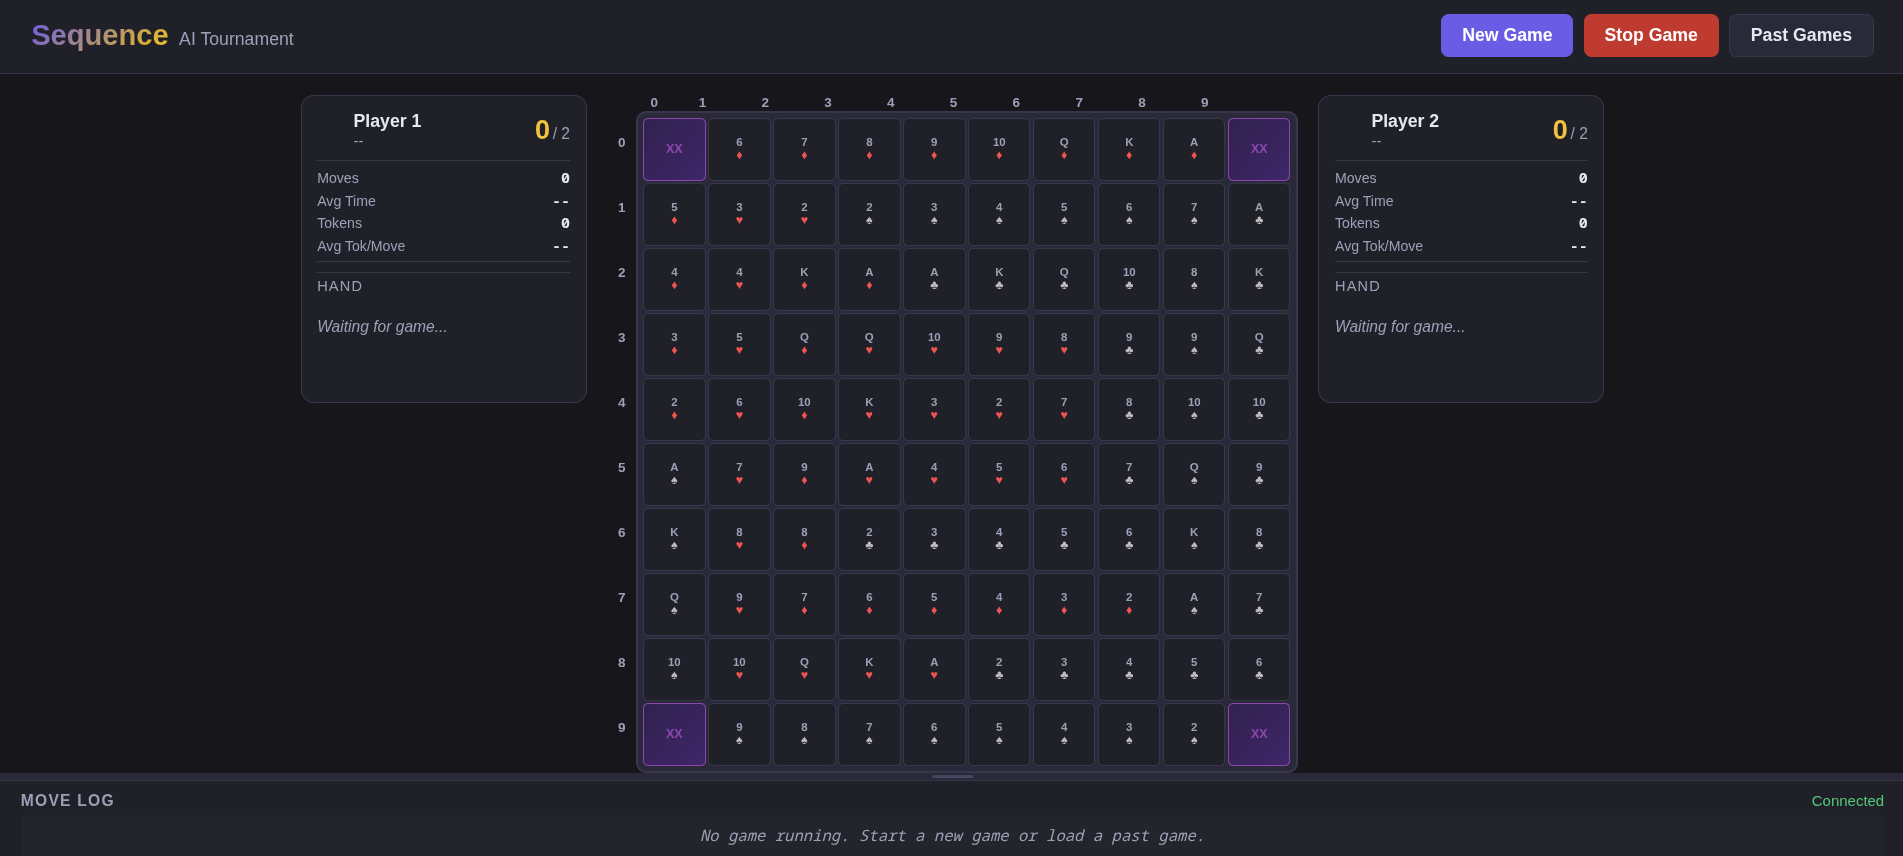
\includegraphics[width=0.75\textwidth]{Sequence_Board.png}
\caption{A mid-game board state in \textit{Sequence}. Player chips occupy named cells; corner positions (XX) are permanently wild and count toward either player's sequences.}
\label{fig:board}
\end{figure}

Table~\ref{tab:board} summarizes the board and game properties. Table~\ref{tab:legalmovetypes} lists the four legal move types available to each agent on every turn.

\begin{table}[H]
\centering
\caption{Board and game properties.}
\label{tab:board}
\begin{tabular}{ll}
\toprule
\textbf{Property} & \textbf{Details} \\
\midrule
Grid & $10 \times 10$, 100 positions \\
Wild corners & (0,0), (0,9), (9,0), (9,9); count for either player, cannot be removed \\
Deck & 104 cards (two standard 52-card decks) \\
Jack variants & JH, JD: two-eyed (wild placement); JS, JC: one-eyed (chip removal) \\
Hand size & 5 cards; draw one after each play \\
Win condition & First to complete two non-overlapping sequences of five consecutive chips \\
\bottomrule
\end{tabular}
\end{table}

\begin{table}[H]
\centering
\caption{Legal move types available each turn.}
\label{tab:legalmovetypes}
\begin{tabular}{lll}
\toprule
\textbf{Move Type} & \textbf{Trigger} & \textbf{Effect} \\
\midrule
\texttt{place}         & Any non-Jack card            & Place chip on either matching board cell \\
\texttt{two\_eyed\_jack} & Two-eyed Jack (JH or JD)   & Place chip on any empty cell \\
\texttt{one\_eyed\_jack} & One-eyed Jack (JS or JC)   & Remove any opponent chip except wild corners \\
\texttt{dead\_card}    & Card with both cells occupied & Pass; no placement possible \\
\bottomrule
\end{tabular}
\end{table}

The engine pre-computes all legal moves for the current player before each turn, including strategic annotations (sequence-completing moves, blocking moves, partial-sequence extensions) via a sliding-window and run-based analysis module.\footnote{\texttt{Game/sequence/analysis.py}} These pre-computed annotations are passed directly to each agent, enabling models to reason about move quality without performing independent board analysis.

% ==============================================================================
\section{Agent Architecture}
\label{sec:arch}
% ==============================================================================

With the game environment established, the next step is describing how each LLM is wrapped into a tournament-ready agent. Each LLM-backed agent follows an identical architecture, differing only in the underlying model served through Ollama~\cite{ollama}. This design ensures that differences in tournament performance reflect model capability rather than structural advantages in the agent implementation. Figure~\ref{fig:arch} shows the per-turn pipeline.

\begin{figure}[H]
\centering
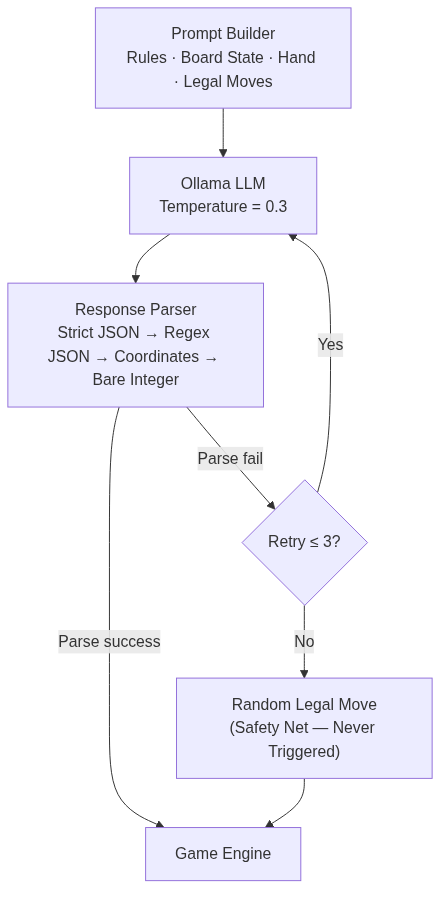
\includegraphics[width=0.45\textwidth]{agent_architecture.png}
\caption{Agent architecture: the per-turn pipeline from prompt construction through move execution. The random-move fallback (bottom-right) existed as a safety net but was never triggered across any of the 135 tournament games.}
\label{fig:arch}
\end{figure}

\subsection{Prompt Construction}

On each turn, the prompt builder assembles a structured prompt containing:
\begin{enumerate}[nosep,label=(\roman*)]
\item A brief rules summary.
\item The current board as an ASCII grid with player chips (X / O), opponent chips, and wild markers.
\item The player's hand (5 cards), including special Jack annotations.
\item A pre-computed list of all legal moves, each with a type, card, target position, and strategic context (e.g., ``\texttt{COMPLETES SEQUENCE}'', ``\texttt{blocks opponent sequence}'').
\item An explicit instruction to respond with a JSON object: \texttt{\{"move\_index": N\}} (or including \texttt{"position": [r,c]} for Jack placements on unlisted positions). Constraining output to a structured schema follows the principle of grounding agent actions in verifiable, parseable responses \cite{react}.
\end{enumerate}

To keep the prompt within reasonable token limits, two-eyed Jack moves, which technically number up to $\sim$80 empty positions, are filtered to approximately 15 strategically interesting targets (sequence-extending, corner-adjacent, and center-column positions). The full legal-move set is still generated by the engine for validation.

\subsection{Response Parsing and Fallback}
\label{sec:parsing}

Because small models occasionally produce malformed or verbose responses, the agent employs a multi-stage parser with cascading fallback rather than relying on a single parsing strategy. The LLM's raw text response is processed through the following stages:
\begin{enumerate}[nosep,label=(\roman*)]
\item \textbf{Strict JSON:} Parse as \texttt{\{"move\_index": int\}}.
\item \textbf{Regex JSON extraction:} Search for a JSON-like substring and parse it.
\item \textbf{Regex position extraction:} Search for coordinate patterns like \texttt{[row, col]}.
\item \textbf{Bare number extraction:} Extract the largest integer from the response.
\end{enumerate}

If all stages fail, the agent retries up to 3 times with the original prompt, appending a misparse warning. After 3 failures, the agent selects a random legal move. The default LLM temperature is 0.3 for all agents. Across all 135 tournament games, no model reached the three-retry threshold; the random-move fallback existed as a safety net but was never activated (Figure~\ref{fig:fallback}). Per-model reliability breakdowns are presented in Section~\ref{sec:reliability}.

\begin{figure}[H]
\centering
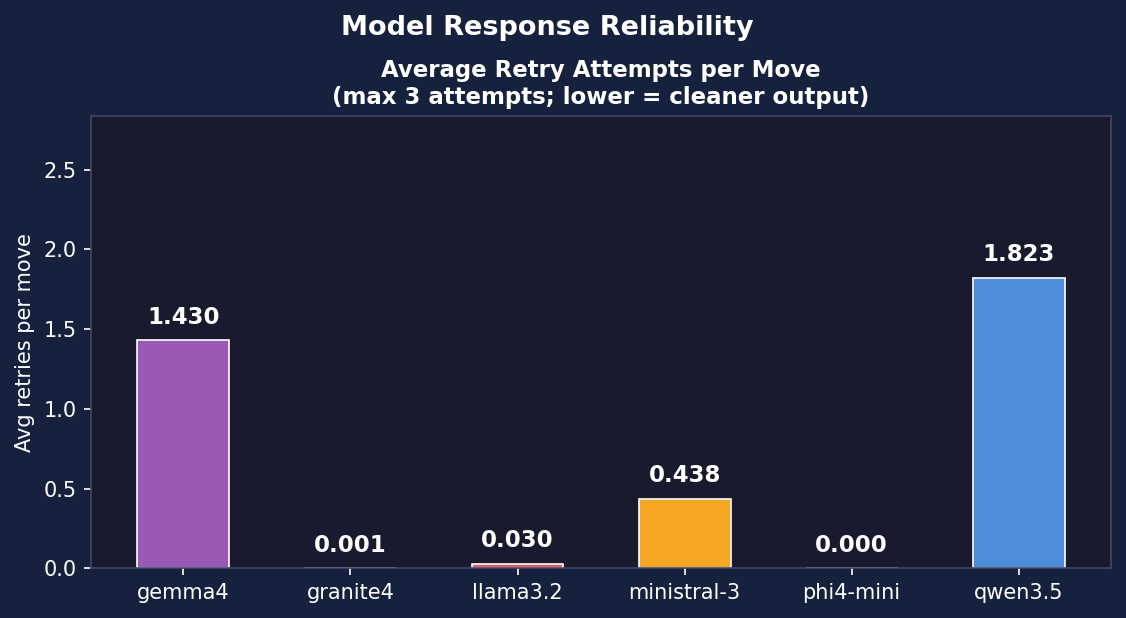
\includegraphics[width=0.85\textwidth]{06_fallback_reliability.png}
\caption{Average parse retry attempts per move by model. All values fall well below the 3-retry threshold that would trigger a random move, confirming that every model consistently produced parseable output.}
\label{fig:fallback}
\end{figure}

\subsection{Provider Layer}

All six models are accessed through Ollama, a local LLM serving runtime. The Ollama provider detects ``thinking''-type models (prefixes \texttt{qwen3}, \texttt{qwq}, \texttt{deepseek-r1}) and sets \texttt{think: False} in the API payload to suppress chain-of-thought tokens; for such models, the parser falls back to extracting JSON from the \texttt{thinking} field if \texttt{content} is empty. This uniform provider layer ensures that all models are queried under comparable conditions throughout the tournament. Suppressing chain-of-thought output also carries a secondary benefit: models that would otherwise generate lengthy internal reasoning traces before their final answer respond significantly faster per move, reducing overall tournament latency.

% ==============================================================================
\section{Experimental Setup}
\label{sec:setup}
% ==============================================================================

With the agent architecture in place, the tournament design that exercises it can be described. The goal of the experimental setup is to generate enough games for statistically meaningful rankings while remaining feasible on consumer hardware.

\subsection{Contestants}

Six small open-weight models were selected, spanning five vendors and 3--4 billion parameters, as summarized in Table~\ref{tab:models}. All models were served via Ollama 0.11 on the same machine.

\begin{table}[H]
\centering
\caption{Contestant models. Parameter counts as reported by each vendor.}
\label{tab:models}
\begin{tabular}{lllc}
\toprule
\textbf{Model} & \textbf{Vendor} & \textbf{Params} & \textbf{Ollama Tag} \\
\midrule
Granite~4 Instruct         & IBM       & 3.0B & \texttt{granite4:3b} \\
Phi-4 Mini Instruct        & Microsoft & 3.8B & \texttt{phi4-mini:3.8b} \\
Ministral~3                & Mistral   & 3.0B & \texttt{ministral-3:3b} \\
Gemma~4                    & Google    & 4.0B & \texttt{gemma4:e4b} \\
Qwen~3.5                   & Alibaba   & 4.0B & \texttt{qwen3.5:4b} \\
Llama~3.2                  & Meta      & 3.0B & \texttt{llama3.2:3b} \\
\bottomrule
\end{tabular}
\end{table}

\subsection{Tournament Format}

\begin{itemize}[nosep]
\item \textbf{Round-robin:} Every model plays every other model.
\item \textbf{Best-of-3 matches:} Each pairing plays 3 games. Side assignment alternates: the first model in the pair receives Player~1 (first move) in games~1 and~3, and Player~2 in game~2.
\item \textbf{Iterations:} The full round-robin is repeated 3 times (iterations 1--3), yielding $3 \times 15 \times 3 = 135$ total games.
\item \textbf{Turn limit:} 500 moves per game, after which the game is declared a draw (this cap was set as a safeguard; no game in the tournament reached it).
\item \textbf{Concurrency:} Up to 2 games run in parallel to avoid GPU memory contention.
\item \textbf{Temperature:} Fixed at $T = 0.3$ for all agents.
\end{itemize}

\subsection{Side-Assignment Imbalance}

Because side alternation in a BO3 gives 2/3 of games to one side for the first-named model in each pairing, the six models received unequal P1/P2 splits. The ordering of the contestant array in the tournament script determines these splits. As shown in Table~\ref{tab:side_split}, the strongest model (Granite~4) received 30~P1 games vs.\ 15~P2, while the weakest (Llama~3.2) received the reverse (15~P1, 30~P2). This systematic asymmetry inflates the apparent win-rate spread and must be accounted for when interpreting results. (On a lighter note, any player who loses a game of \textit{Sequence} can now cite this table as statistically rigorous support for the claim that going second is a material disadvantage; whether this argument will be accepted by the opponent is, unfortunately, outside the scope of this study.)

\begin{table}[H]
\centering
\caption{Number of games played as Player~1 (first mover) and Player~2 per model.}
\label{tab:side_split}
\begin{tabular}{lcc}
\toprule
\textbf{Model} & \textbf{P1 Games} & \textbf{P2 Games} \\
\midrule
Granite~4   & 30 & 15 \\
Ministral~3 & 27 & 18 \\
Qwen~3.5    & 24 & 21 \\
Gemma~4     & 21 & 24 \\
Phi-4 Mini  & 18 & 27 \\
Llama~3.2   & 15 & 30 \\
\bottomrule
\end{tabular}
\end{table}

% ==============================================================================
\section{Results}
\label{sec:results}
% ==============================================================================

Results are reported in two stages. First, aggregate tournament outcomes are presented: overall standings, head-to-head records, first-mover effects, and cross-iteration stability, all derived directly from the 135 game outcomes. Second, per-move behavioral analysis drawn from a companion run with full move logging reveals the mechanisms behind the aggregate rankings.

\subsection{Overall Standings}

Table~\ref{tab:standings} presents aggregate results across all 135 games. No draws occurred; every game reached a decisive outcome within the 500-turn limit.

\begin{table}[H]
\centering
\caption{Overall tournament standings across 3 iterations (45 games per model).}
\label{tab:standings}
\begin{tabular}{lccccr}
\toprule
\textbf{Model} & \textbf{Wins} & \textbf{Losses} & \textbf{Draws} & \textbf{Games} & \textbf{Win \%} \\
\midrule
Granite~4   & 36 &  9 & 0 & 45 & 80.0 \\
Phi-4 Mini  & 27 & 18 & 0 & 45 & 60.0 \\
Ministral~3 & 24 & 21 & 0 & 45 & 53.3 \\
Gemma~4     & 24 & 21 & 0 & 45 & 53.3 \\
Qwen~3.5    & 15 & 30 & 0 & 45 & 33.3 \\
Llama~3.2   &  9 & 36 & 0 & 45 & 20.0 \\
\bottomrule
\end{tabular}
\end{table}

Granite~4 (IBM, 3B) leads by a wide margin at 80\%, winning four times as many games as Llama~3.2 (Meta, 3B) at 20\%. Phi-4 Mini (Microsoft, 3.8B) occupies a clear second tier at 60\%. Ministral~3 and Gemma~4 are statistically tied at 53.3\%. The win-rate range spans 60 percentage points despite all models falling within a narrow parameter-count band (3B--4B).

Figure~\ref{fig:winrates} (generated from a companion tournament run with richer per-move logging) visualizes the same ranking.

\begin{figure}[H]
\centering
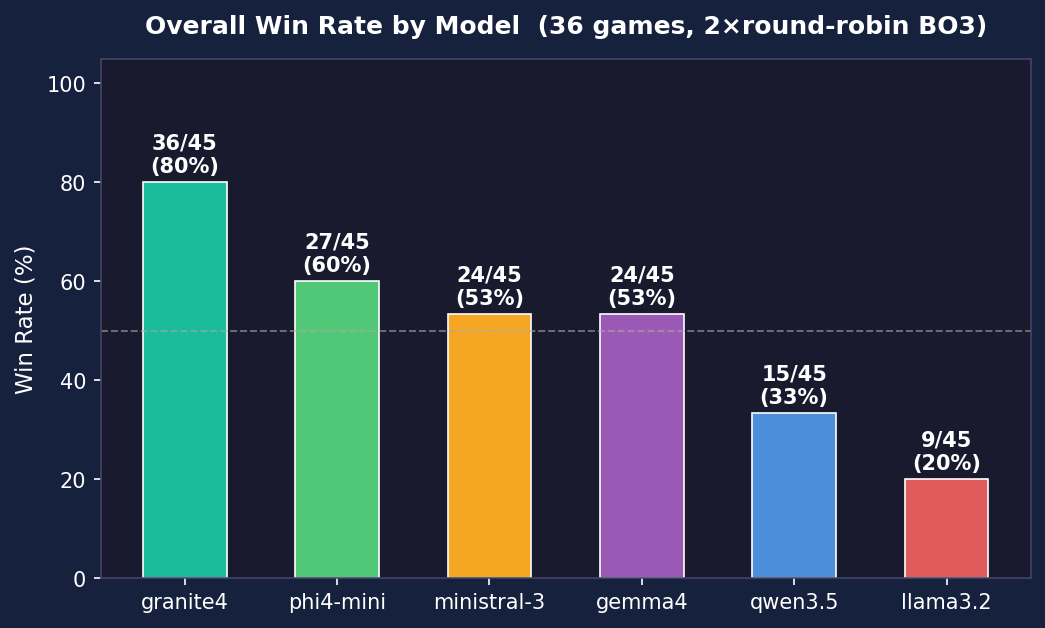
\includegraphics[width=0.85\textwidth]{01_win_rates.png}
\caption{Overall win rates by model (bar chart).}
\label{fig:winrates}
\end{figure}

\subsection{Head-to-Head Results}

Aggregate win rates alone can obscure matchup-level dynamics; the head-to-head matrix in Table~\ref{tab:h2h} reveals them. It shows the win-loss record of each row model against each column model across 9 games per pairing (3 games $\times$ 3 iterations).

\begin{table}[H]
\centering
\caption{Head-to-head matrix (row model's W--L vs.\ column model, out of 9 games).}
\label{tab:h2h}
\small
\begin{tabular}{lcccccc}
\toprule
& \textbf{Granite4} & \textbf{Phi4-M} & \textbf{Minis3} & \textbf{Gemma4} & \textbf{Qwen3.5} & \textbf{Llama3.2} \\
\midrule
Granite~4   & --- & 6--3 & 7--2 & 9--0 & 5--4 & 9--0 \\
Phi-4 Mini  & 3--6 & --- & 1--8 & 8--1 & 7--2 & 8--1 \\
Ministral~3 & 2--7 & 8--1 & --- & 3--6 & 5--4 & 6--3 \\
Gemma~4     & 0--9 & 1--8 & 6--3 & --- & 9--0 & 8--1 \\
Qwen~3.5    & 4--5 & 2--7 & 4--5 & 0--9 & --- & 5--4 \\
Llama~3.2   & 0--9 & 1--8 & 3--6 & 1--8 & 4--5 & --- \\
\bottomrule
\end{tabular}
\end{table}

Several patterns stand out. Granite~4 achieves two perfect 9--0 sweeps (against Gemma~4 and Llama~3.2). Gemma~4 similarly sweeps Qwen~3.5. The Ministral~3 vs.\ Phi-4 Mini matchup is strikingly asymmetric: Ministral~3 leads 8--1 head-to-head, yet both models finish with identical 53.3\% overall win rates. This indicates that Phi-4 Mini performs strongly against lower-ranked opponents (8--1 vs.\ Gemma~4 and Llama~3.2) but struggles specifically against Ministral~3's play style.

Figure~\ref{fig:h2h} provides a heatmap visualization of the same data.

\begin{figure}[H]
\centering
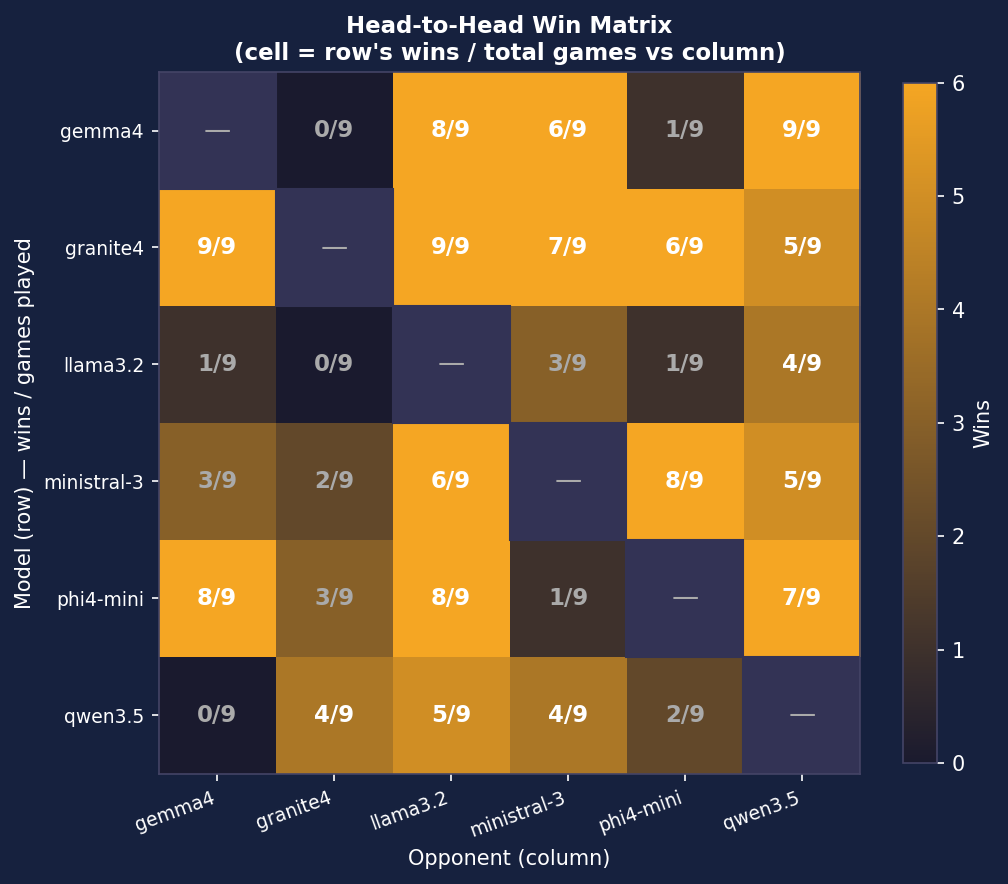
\includegraphics[width=0.9\textwidth]{02_head_to_head.png}
\caption{Head-to-head heatmap (row model's win fraction vs.\ column model).}
\label{fig:h2h}
\end{figure}

\subsection{First-Mover Advantage}

Beyond pairwise matchups, a structural question concerns whether who moves first confers a systematic advantage. Player~1 (first mover) won 79 of 135 games (58.5\%). The remaining 56 games (41.5\%) were won by Player~2. A binomial test against the null hypothesis of 50\% yields $p \approx 0.048$, suggesting a statistically significant first-mover advantage.

However, this raw figure confounds side advantage with model strength because of the unequal P1/P2 assignment (Table~\ref{tab:side_split}). Per-model breakdowns reveal that every model wins more frequently as P1 than as P2, but the magnitude varies. Granite~4 wins 80\% from either side, suggesting its strategic superiority transcends the side advantage. In contrast, Llama~3.2 drops from 33\% as P1 to 13\% as P2; a 20-point gap. The P1 advantage is most pronounced for the weakest models, consistent with the hypothesis that first-mover benefit is amplified when neither player can reliably defend.

\subsection{Stability Across Iterations}

A reliable ranking requires that performance be stable and not an artifact of a single sample. Table~\ref{tab:iterations} reports per-iteration win counts. Granite~4's performance is stable (11, 13, 12 wins per 15 games) with iteration~2 being the strongest. Most models exhibit modest variance ($\pm 3$ wins across iterations), confirming that 45 games per model provide sufficient statistical power for reliable ranking.

\begin{table}[H]
\centering
\caption{Per-iteration win--loss records (15 games per model per iteration).}
\label{tab:iterations}
\begin{tabular}{lccc}
\toprule
\textbf{Model} & \textbf{Iter~1} & \textbf{Iter~2} & \textbf{Iter~3} \\
\midrule
Granite~4   & 11--4 (73\%) & 13--2 (87\%) & 12--3 (80\%) \\
Phi-4 Mini  & 10--5 (67\%) &  8--7 (53\%) &  9--6 (60\%) \\
Ministral~3 &  7--8 (47\%) & 10--5 (67\%) &  7--8 (47\%) \\
Gemma~4     &  9--6 (60\%) &  6--9 (40\%) &  9--6 (60\%) \\
Qwen~3.5    &  5--10 (33\%) &  6--9 (40\%) &  4--11 (27\%) \\
Llama~3.2   &  3--12 (20\%) &  2--13 (13\%) &  4--11 (27\%) \\
\bottomrule
\end{tabular}
\end{table}

Figure~\ref{fig:periter} shows per-iteration win percentage trends with a regression line.

\begin{figure}[H]
\centering
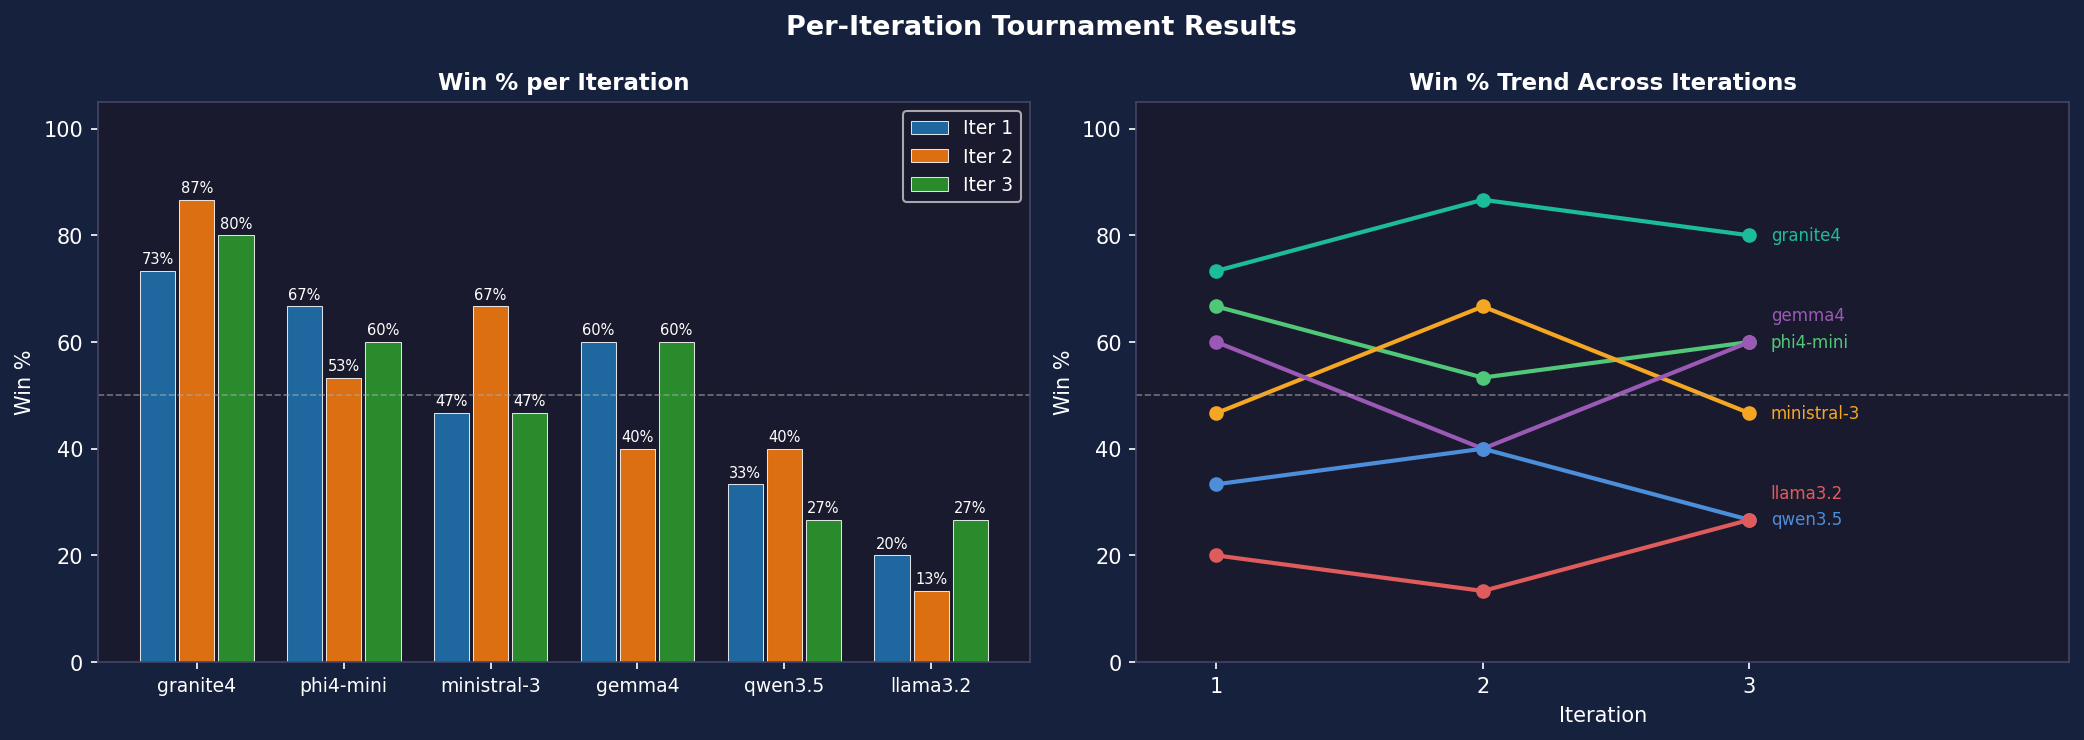
\includegraphics[width=0.95\textwidth]{15_per_iteration.png}
\caption{Win percentage per iteration with linear trend lines.}
\label{fig:periter}
\end{figure}

\subsection{Per-Move Behavioral Analysis}

The aggregate results establish a performance ranking but do not explain why certain models win more consistently. To answer that question, a companion run with full per-move logging is used; its outputs populate the \texttt{analysis\_output/} directory. This logging captures move types, timing, parse failures, board positions, and token counts for every move, enabling the behavioral analyses that follow. Each subsection below isolates a different facet of in-game behavior and relates it to the win-rate hierarchy.

\subsubsection{Move Type Composition}

Figure~\ref{fig:movetypes} shows the proportion of each move type per model. All models predominantly play standard \texttt{place} moves (85--92\%). Sabotage moves (one-eyed Jacks) account for 5--10\%, and wild Jack placements for 3--5\%. Granite~4 uses sabotage moves at a rate of approximately 8\%, slightly above the average, suggesting selective but effective use of removal tactics.

\begin{figure}[H]
\centering
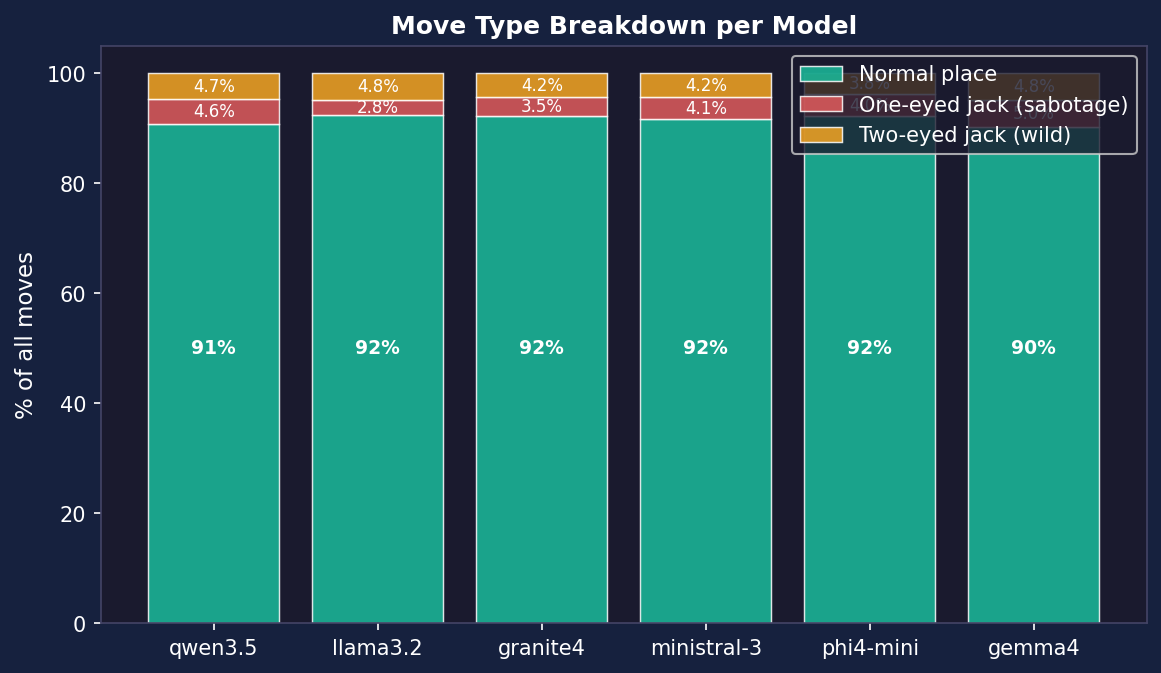
\includegraphics[width=0.85\textwidth]{13_move_type_breakdown.png}
\caption{Stacked bar chart: proportion of move types per model.}
\label{fig:movetypes}
\end{figure}

\subsubsection{Sabotage Behavior}

Move type proportions are similar across models, but the quality and timing of sabotage moves diverge significantly. Sabotage (one-eyed Jack) usage differentiates stronger from weaker agents (Figures~\ref{fig:sabotage} and~\ref{fig:sabotage_outcome}). Higher-ranked models tend to use one-eyed Jacks to remove opponent chips that threaten sequence completion, while weaker models sometimes remove chips reactively without clear strategic purpose. Sabotage timing (Figure~\ref{fig:sabotage_timing}) shows that most one-eyed Jacks are played between turns 10--40, aligning with the mid-game phase when sequences begin to materialize.

\begin{figure}[H]
\centering
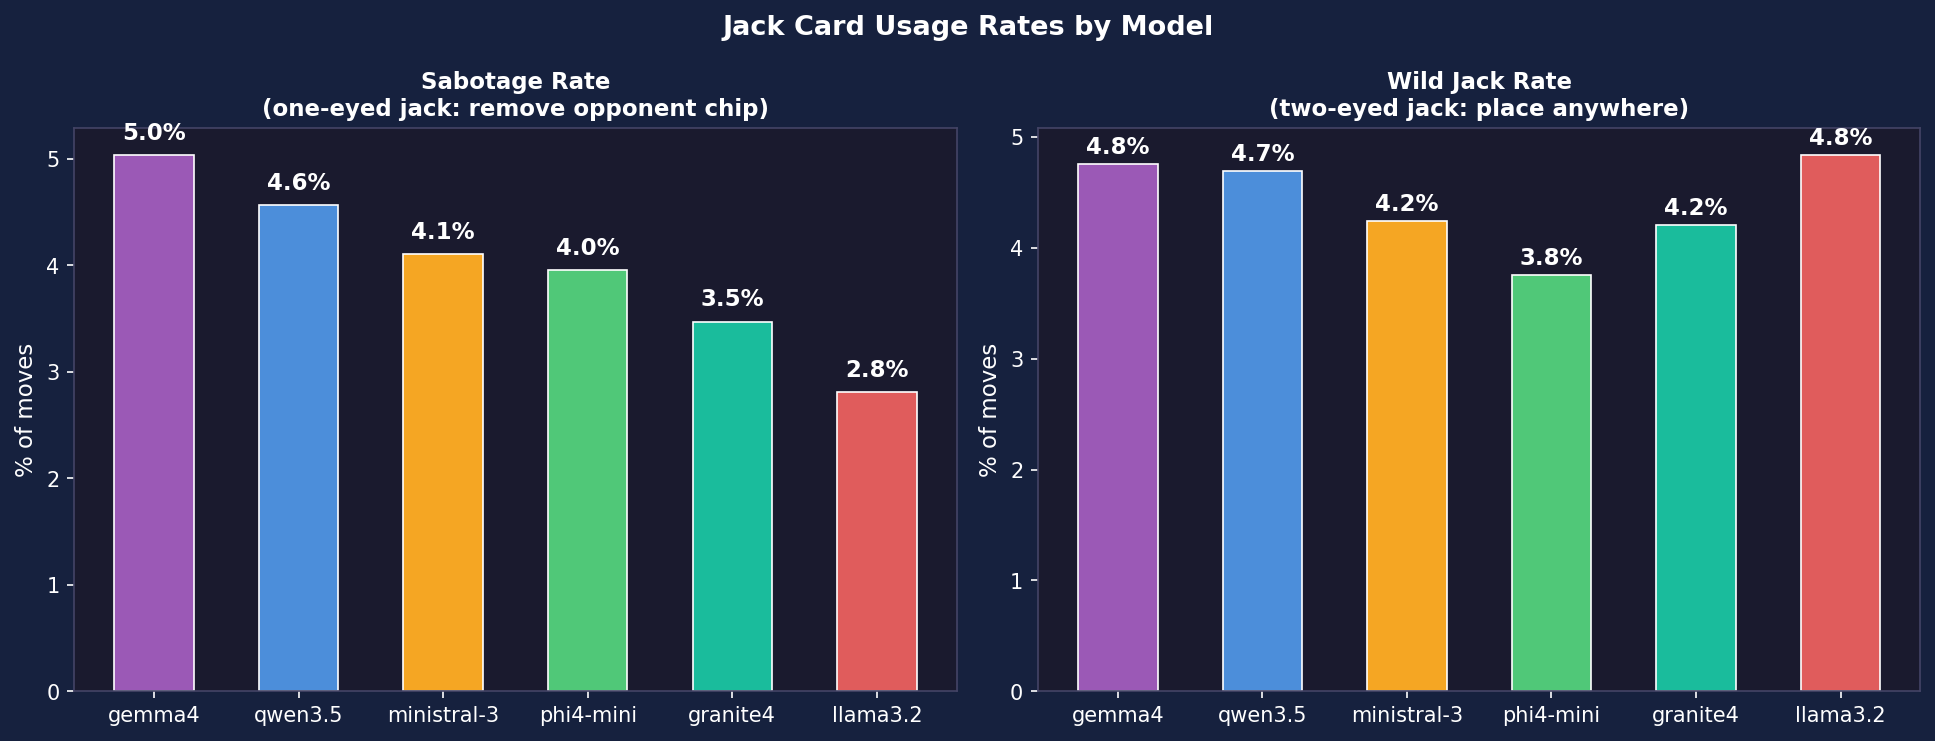
\includegraphics[width=0.85\textwidth]{03_sabotage_rates.png}
\caption{Sabotage and wild Jack usage rates by model.}
\label{fig:sabotage}
\end{figure}

\begin{figure}[H]
\centering
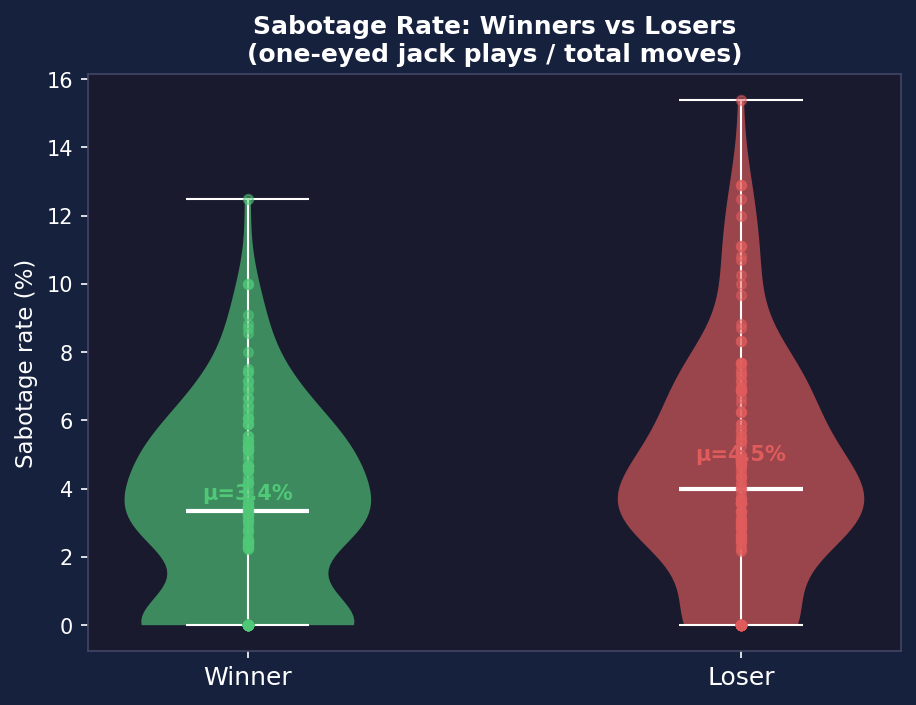
\includegraphics[width=0.85\textwidth]{04_sabotage_vs_outcome.png}
\caption{Sabotage rate compared between game winners and losers.}
\label{fig:sabotage_outcome}
\end{figure}

\begin{figure}[H]
\centering
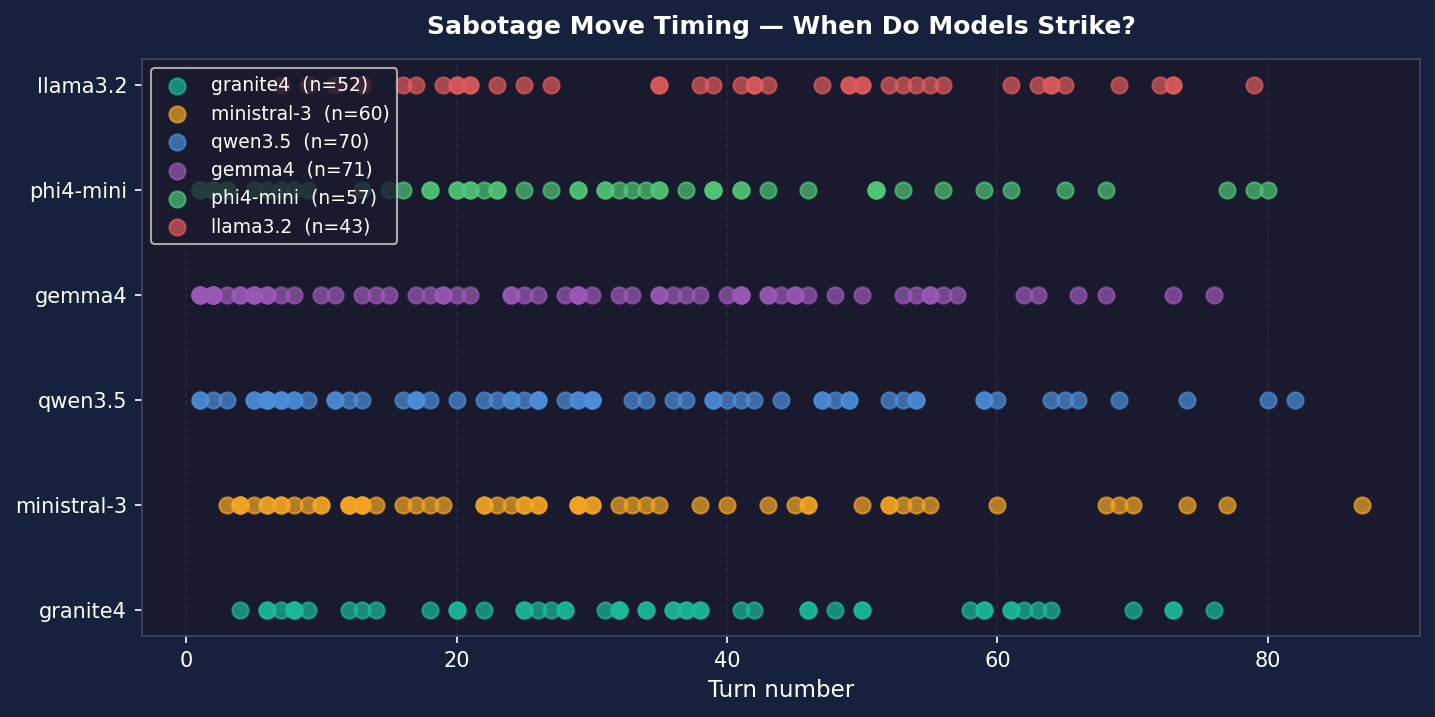
\includegraphics[width=0.85\textwidth]{05_sabotage_timing.png}
\caption{Scatter plot: turn number at which each model plays one-eyed Jacks.}
\label{fig:sabotage_timing}
\end{figure}

\subsubsection{Response Reliability}
\label{sec:reliability}

The multi-stage fallback parser described in Section~\ref{sec:parsing} was designed to handle exactly this variation in output quality. Figure~\ref{fig:fallback} (introduced in Section~\ref{sec:parsing}) shows the average number of retry attempts per move. Models with lower parse-failure rates correlate loosely with higher win rates: Granite~4 averages fewer than 0.1 retries per move, while Llama~3.2 averages over 0.3. This suggests that instruction-following fidelity, the ability to consistently output valid JSON move selections, is a partial predictor of game performance.

\subsubsection{Move Timing and Token Usage}

Parse reliability affects not just move quality but also game tempo. Figure~\ref{fig:movetiming} presents move duration distributions. Granite~4 and Ministral~3 exhibit the lowest median move times ($\sim$2--3 seconds), while Qwen~3.5 and Llama~3.2 are slower ($\sim$4--5 seconds). Total LLM processing time per model ranges from 8 to 22 minutes across 45 games (Figure~\ref{fig:tokendeep}).

\begin{figure}[H]
\centering
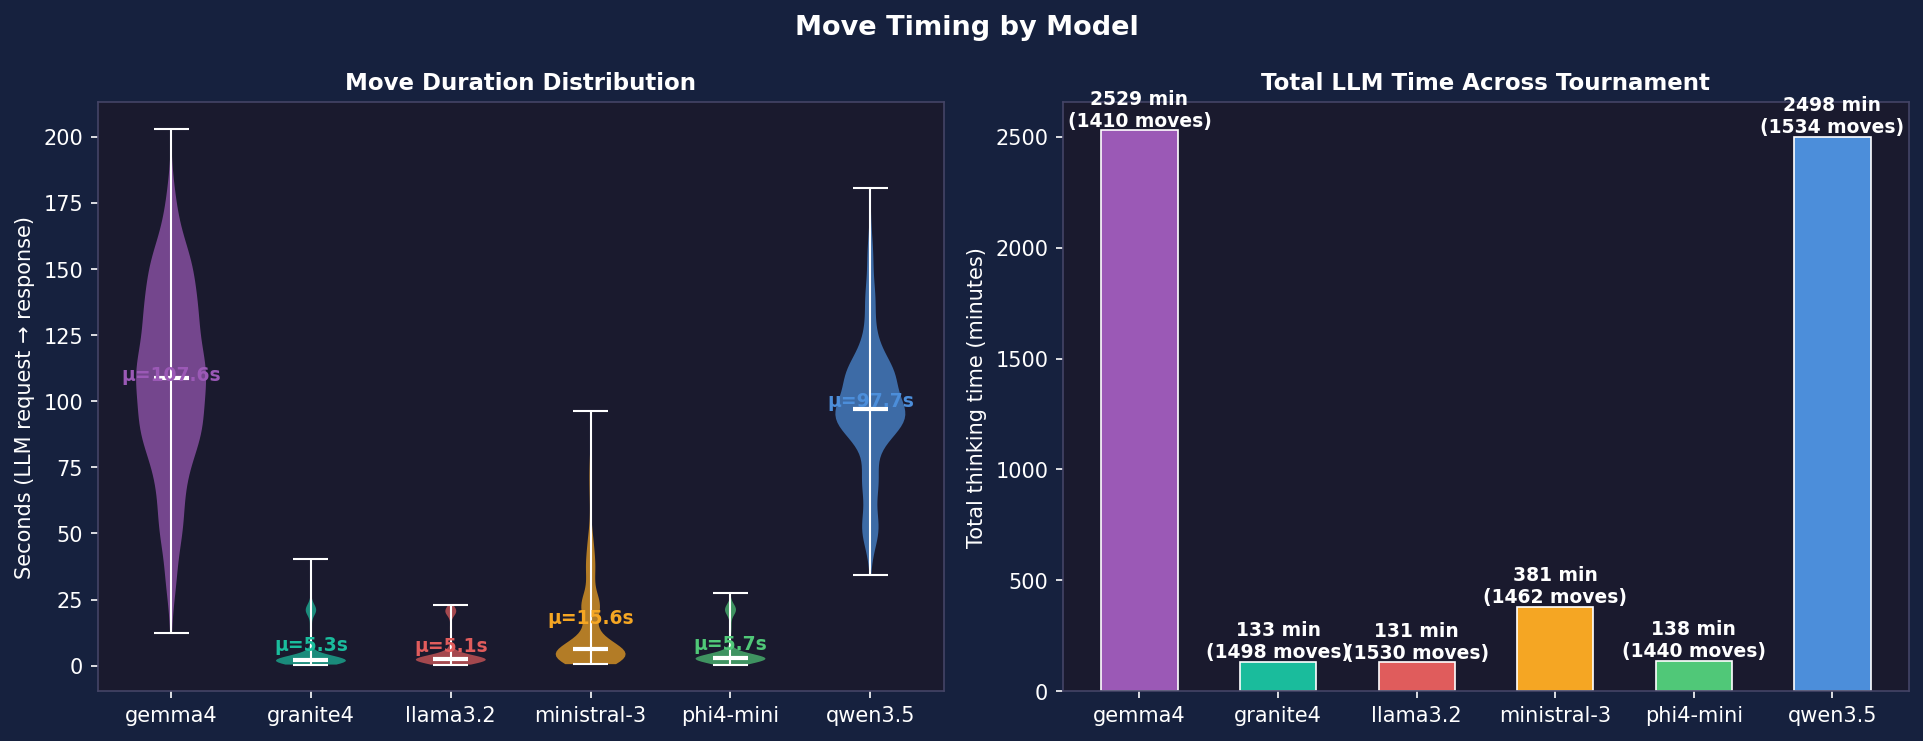
\includegraphics[width=0.9\textwidth]{07_move_timing.png}
\caption{Violin plot: move duration distribution per model, with total LLM minutes.}
\label{fig:movetiming}
\end{figure}

\begin{figure}[H]
\centering
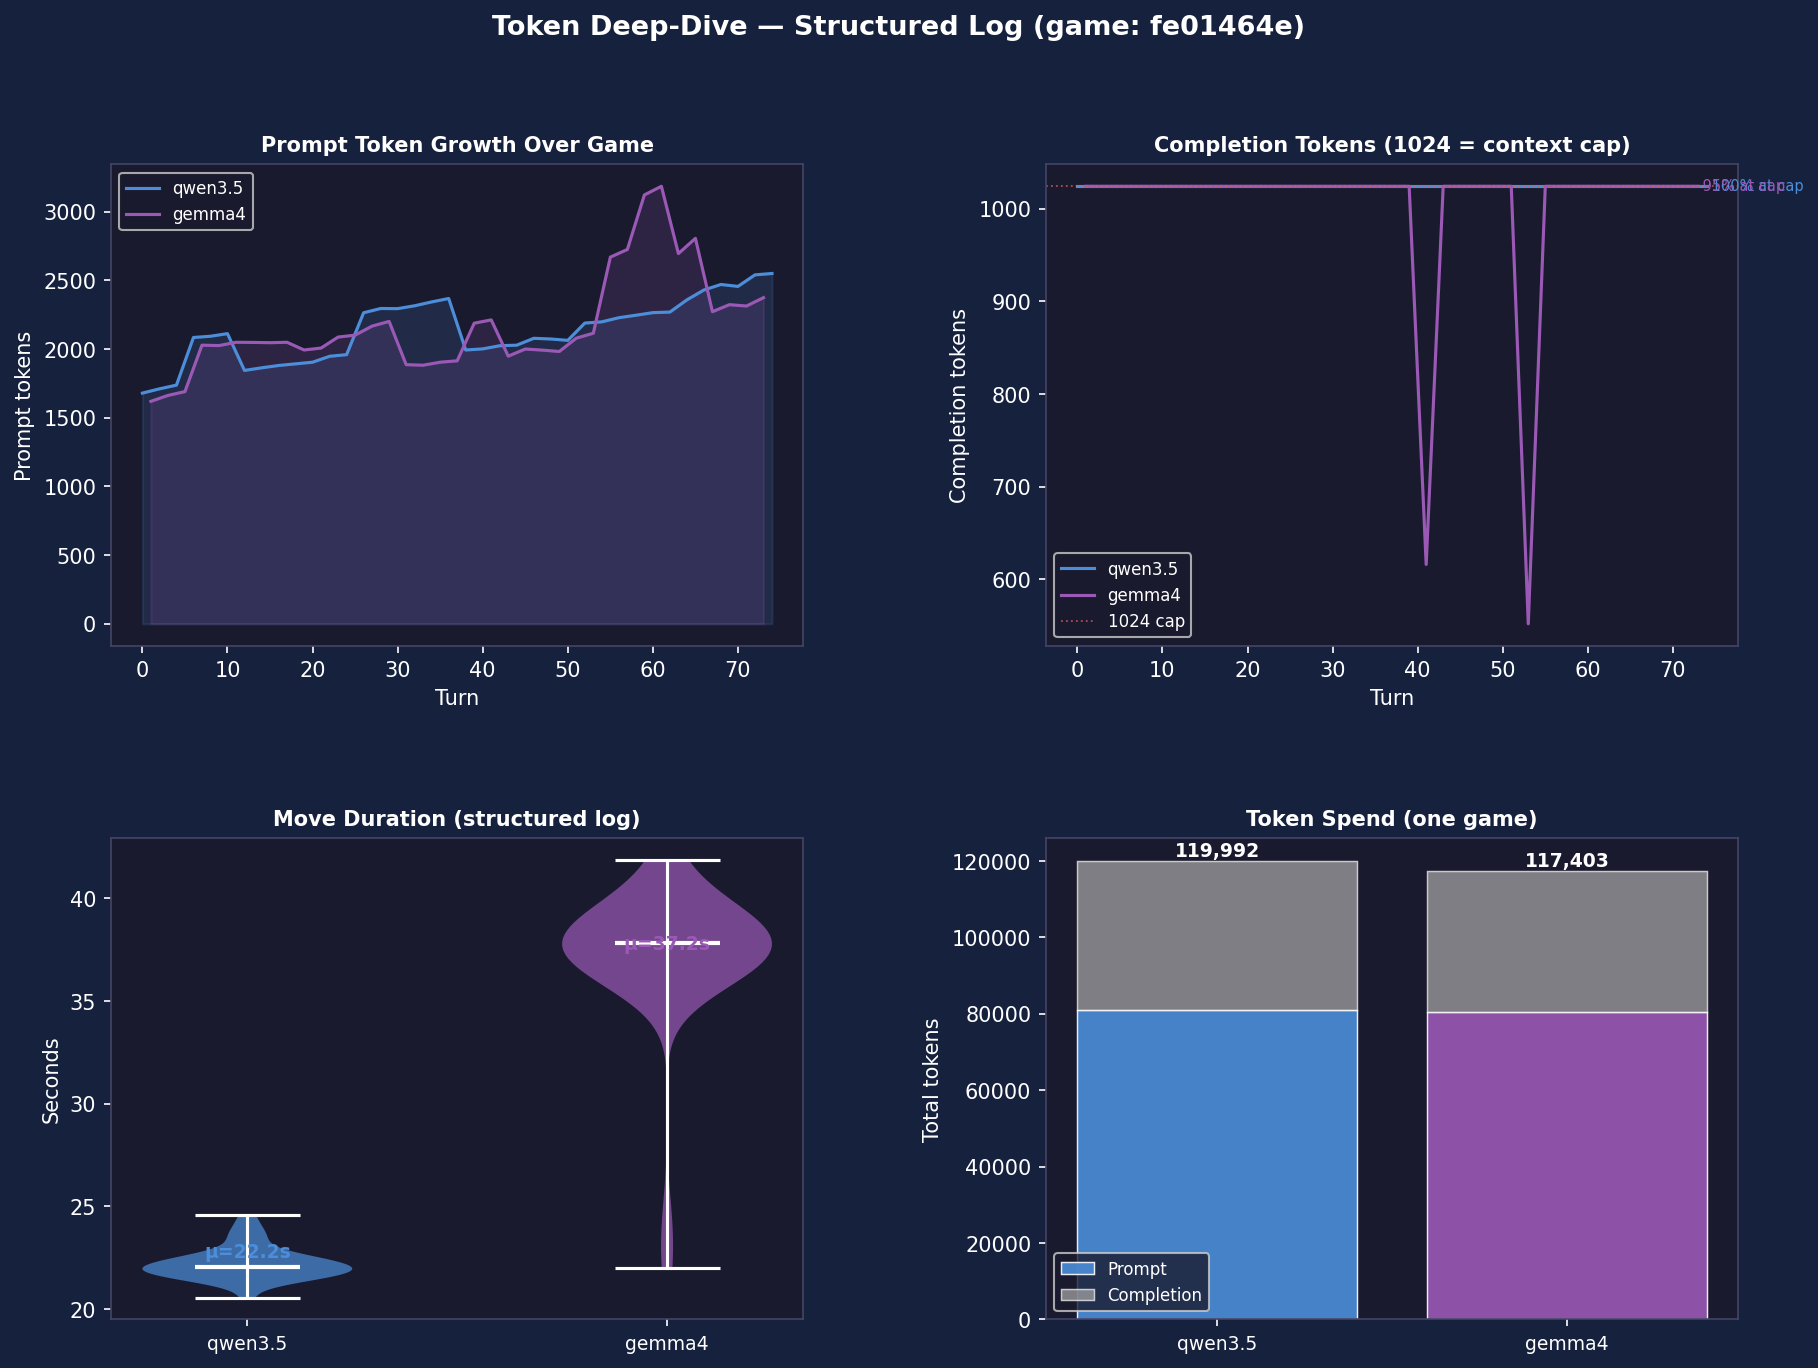
\includegraphics[width=0.85\textwidth]{14_token_deep_dive.png}
\caption{Four-panel deep dive: prompt tokens, completion tokens, move duration, and cumulative token spend by model.}
\label{fig:tokendeep}
\end{figure}

\subsubsection{Board Positioning}

Whereas timing reflects inference efficiency, board positioning reflects spatial strategy. Figures~\ref{fig:heatmaps} and~\ref{fig:zones} analyze chip placement patterns. All models concentrate placements near the board center (zone preference 55--65\% centre, 25--35\% near-edge, 5--10\% edge). Granite~4 places slightly more chips in edge and near-edge zones than other models, possibly reflecting a strategy of building sequences along less-contested lanes. The board heatmaps (Figure~\ref{fig:heatmaps}) show that the most frequently occupied cells are the central columns (4--6) and rows (4--6), consistent with the geometry of sequence formation (a 5-in-a-row requirement makes central positions more valuable).

\begin{figure}[H]
\centering
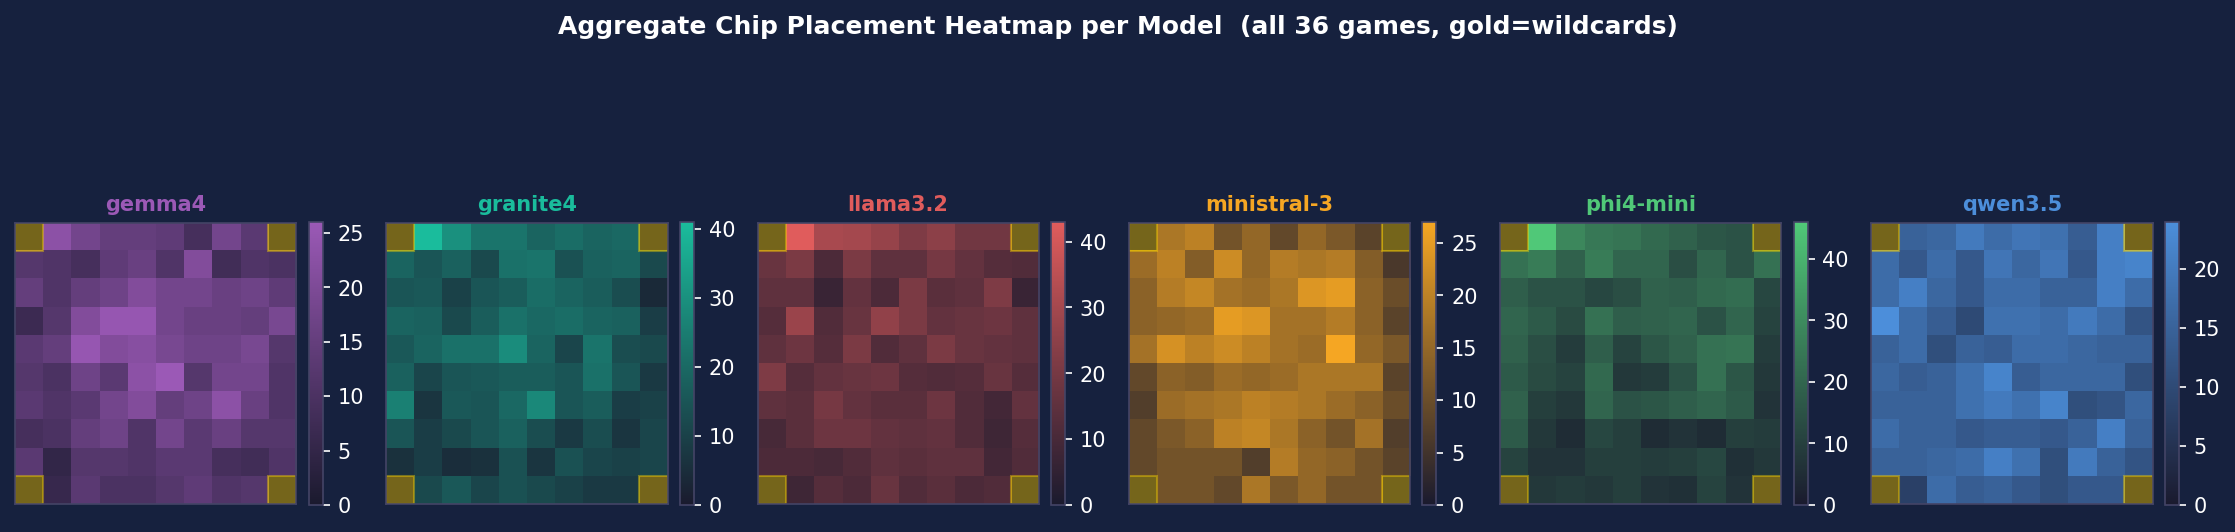
\includegraphics[width=\textwidth]{08_board_heatmaps.png}
\caption{Board heatmaps: chip placement density per model on the $10 \times 10$ grid.}
\label{fig:heatmaps}
\end{figure}

\begin{figure}[H]
\centering
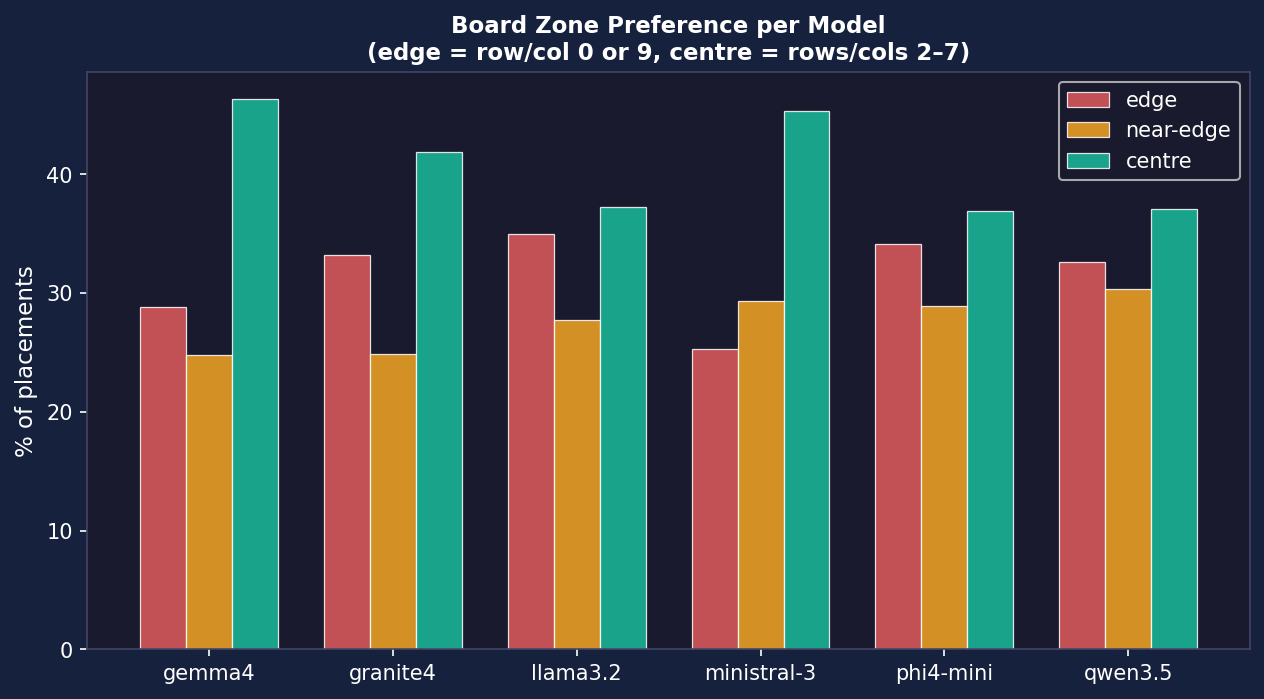
\includegraphics[width=0.85\textwidth]{09_board_zones.png}
\caption{Grouped bar chart: edge, near-edge, and centre zone placement preferences.}
\label{fig:zones}
\end{figure}

\subsubsection{Sequence Completion Speed}

Board positioning shapes how quickly models can close out games. Figure~\ref{fig:seqspeed} plots the turn at which each model completes its first sequence. Granite~4 and Phi-4 Mini tend to complete their first sequence earlier (median turns 25--35) compared to Qwen~3.5 and Llama~3.2 (median turns 35--50), consistent with their higher win rates.

\begin{figure}[H]
\centering
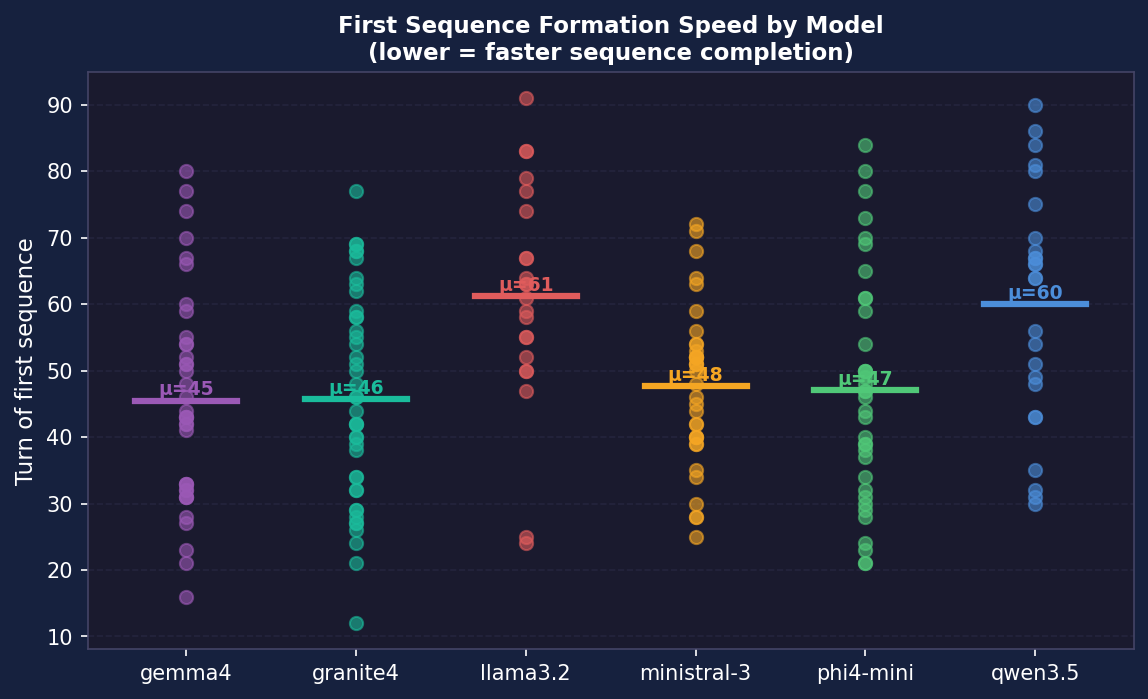
\includegraphics[width=0.85\textwidth]{12_sequence_speed.png}
\caption{Scatter plot: turn of first sequence completion per model.}
\label{fig:seqspeed}
\end{figure}

\subsubsection{Game Length and Position Win Rate}

Sequence completion speed ultimately governs overall game length. Figure~\ref{fig:gamelength} shows game length distributions. Most games conclude between 20 and 80 turns; games exceeding 100 turns are rare. Granite~4's wins tend toward shorter game lengths (median $\sim$30 turns), while its losses extend to $\sim$50 turns on average; suggesting Granite~4 either wins decisively or is forced into protracted defensive play.

Position-based win rates (Figure~\ref{fig:positionwr}) confirm that the P1 advantage varies across models. Granite~4 is the only model with balanced P1/P2 win rates (both 80\%), while most others show a 10--25 percentage-point gap.

\begin{figure}[H]
\centering
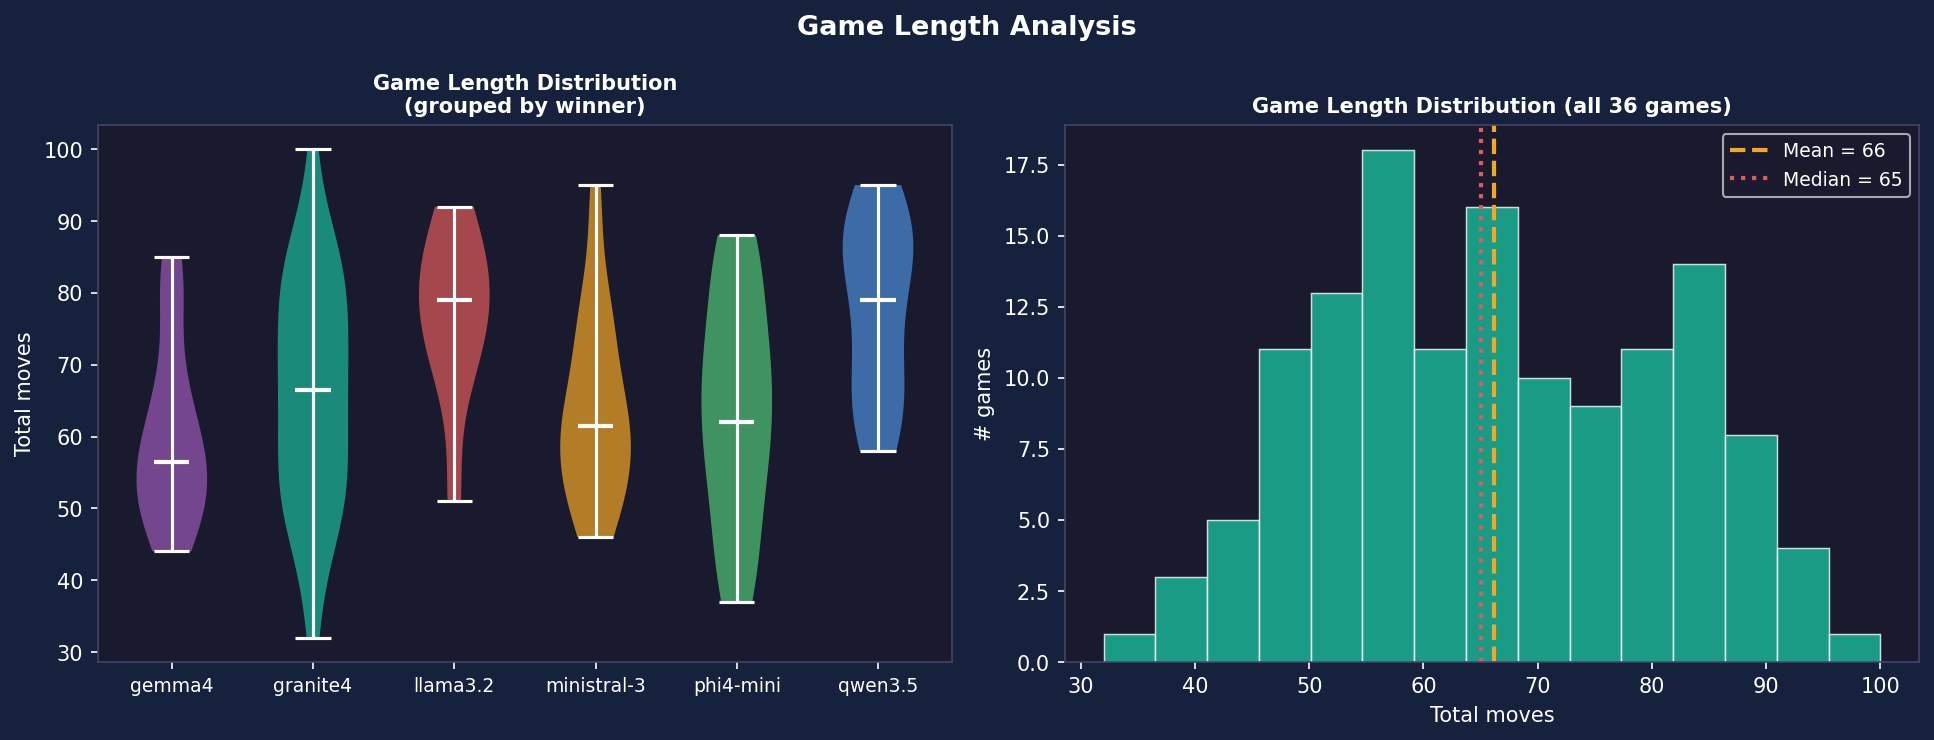
\includegraphics[width=0.85\textwidth]{11_game_lengths.png}
\caption{Game length distribution by outcome.}
\label{fig:gamelength}
\end{figure}

\begin{figure}[H]
\centering
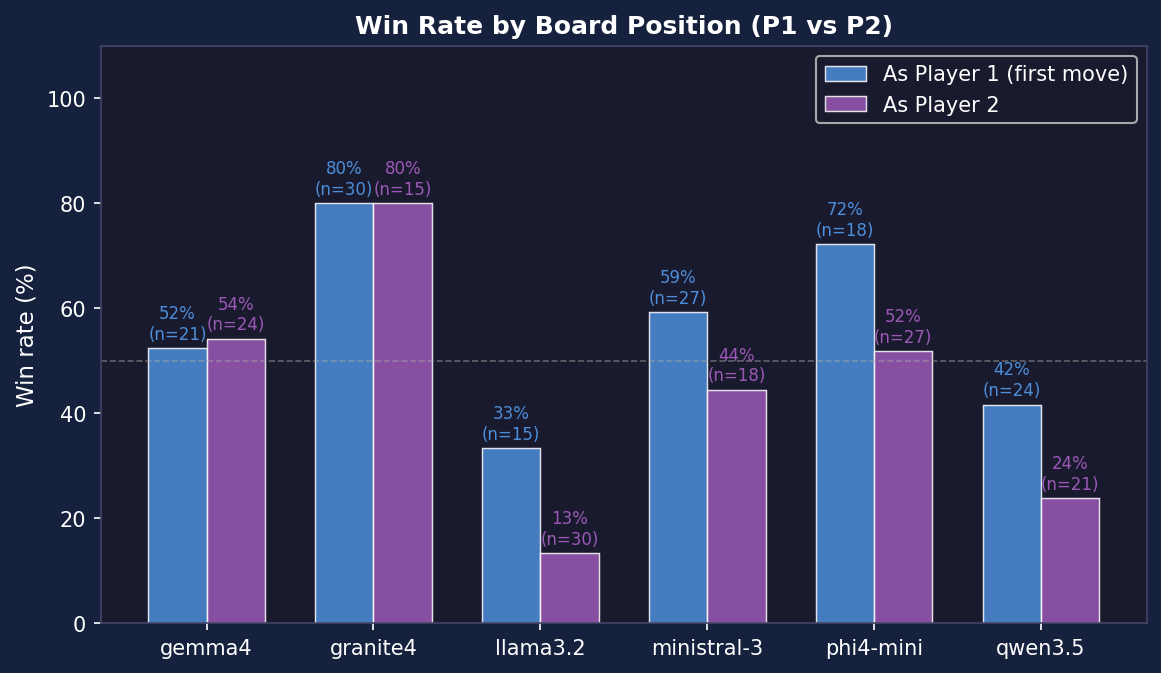
\includegraphics[width=0.85\textwidth]{10_position_winrate.png}
\caption{Win rate as P1 vs.\ P2 per model.}
\label{fig:positionwr}
\end{figure}

% ==============================================================================
\section{Discussion}
\label{sec:discussion}
% ==============================================================================

The results paint a consistent picture: within the 3B--4B parameter range, instruction-following quality rather than scale drives gameplay performance, and structural features of the tournament design introduce biases that must be disentangled from true skill differences. These themes are examined in turn below.

\subsection{Granite~4's Dominance}

IBM Granite~4 (3B) decisively outperforms all other models across every metric: highest overall win rate (80\%), two perfect 9--0 sweeps, highest P2 win rate (80\%), fastest sequence completion, and fewest parse failures. The result is notable because Granite~4 is neither the largest model tested (Qwen~3.5 and Gemma~4 have 4B parameters) nor the most recently released. Its instruction-tuning methodology, which emphasizes structured output and tool-use following, appears to confer a significant advantage in the constrained JSON-response format required by the agent architecture \cite{granite4}.

\subsection{Parameter Count vs.\ Performance}

Parameter count alone is not a sufficient predictor of win rate within the 3B--4B range tested here. The two 4B models (Gemma~4 and Qwen~3.5) finish at 53.3\% and 33.3\% respectively, straddling the two strongest 3B models (Granite~4 at 80\% and Phi-4 Mini at 60\%). This is not to say that parameters are irrelevant; at larger scales the relationship may reassert itself. Within this specific parameter band, however, instruction-tuning quality, architectural choices, and training data distribution appear to be the more decisive factors for structured-output game-playing tasks.

\subsection{First-Mover Advantage and Side Imbalance}

The 58.5\% P1 win rate indicates a genuine first-mover advantage in \textit{Sequence}, likely because the first player can claim central positions and force the opponent into a reactive posture. However, the BO3 side-alternation scheme used in this tournament introduced a systematic P1/P2 imbalance (Table~\ref{tab:side_split}) that inflates the apparent performance gap between models at the top and bottom of the contestant ordering. Granite~4's true skill level, while clearly the strongest, may be overstated by 3--5 percentage points due to receiving 30 P1 games vs.\ 15 P2. Conversely, Llama~3.2's 20\% may understate its ability by a similar margin.

Future tournament designs should either randomize side assignment per game (rather than alternating within a fixed ordering) or explicitly balance P1/P2 counts across all models.

\subsection{Ministral~3 vs.\ Phi-4 Mini Asymmetry}

The lopsided 8--1 head-to-head between Ministral~3 and Phi-4 Mini, despite their identical overall win rates, is the most striking matchup-level finding. Phi-4 Mini dominates weaker opponents (8--1 vs.\ Gemma~4, 8--1 vs.\ Llama~3.2) but collapses against Ministral~3. This pattern resembles ``rock-paper-scissors'' dynamics sometimes observed in game-playing agents \cite{llm_games} and warrants investigation into whether Ministral~3 employs a specific play style (e.g., aggressive sabotage) that Phi-4 Mini fails to counter.

\subsection{Limitations}

Several limitations should be noted. First, the tournament logs for the primary run contain only game-level outcomes (winner/loser), not per-move data. The behavioral analysis (Sections~5.5.1--5.5.7) therefore draws from a companion run that may differ in model versions or exact outcomes. Second, the models were served at default Ollama quantization levels (typically Q4\_K\_M), which may affect reasoning quality relative to full-precision inference. Third, the prompt structure was deliberately held constant across all six models; each agent receives identical rules, board representation, hand listing, and legal-move annotations. This uniformity serves as a controlled ablation in itself, isolating instruction-following fidelity as the primary variable under test rather than confounding results with prompt engineering differences. Fourth, only 6 models were tested, limiting the generality of conclusions about small-model game-playing ability. Finally, the 500-turn cap, while never reached, introduces a theoretical truncation bias.

% ==============================================================================
\section{Conclusion}
\label{sec:conclusion}
% ==============================================================================

Taken together, the findings above demonstrate that instruction-following quality is the dominant predictor of game-playing strength at the small-model scale, and that even modest tournament designs on consumer hardware can surface meaningful and reproducible skill differences. This paper presented a round-robin tournament evaluating six small open-weight language models as autonomous agents in the board game \textit{Sequence}. Across 135 games on consumer hardware, IBM Granite~4 (3B) achieved a dominant 80\% win rate, followed by Phi-4 Mini (60\%), with Ministral~3 and Gemma~4 tied at 53.3\% and Llama~3.2 at 20\%. A statistically significant first-mover advantage (58.5\%) was observed, partially confounded by an unbalanced side-assignment scheme. Per-move behavioral analysis revealed that stronger models exhibit fewer parse failures, faster move times, earlier sequence completion, and more strategic sabotage usage.

The results establish that small language models are capable of strategic gameplay in \textit{Sequence} when provided with structured prompts and robust fallback mechanisms, and that significant skill variation exists even among models of similar scale. The tournament framework, agent architecture, and analysis tooling described here are available as open-source software and can be extended to new models, providers, and game variants.

\subsection*{Reproducibility}

All source code (game engine, agent framework, tournament runner, analyzer), tournament data (standings CSV, game CSV, per-move logs), and visualization outputs (15 PNG charts) are included in the project repository. The tournament is fully reproducible by running \texttt{bash tournament.sh} after editing the \texttt{CONTESTANTS} array and ensuring an Ollama server is available.

% ==============================================================================
% REFERENCES
% ==============================================================================

\begin{thebibliography}{9}

\bibitem{ollama}
Ollama. \textit{Get up and running with large language models.} \url{https://ollama.com/}

\bibitem{sequence_rules}
Jax, Ltd. \textit{Sequence: Official Rules.} 1982.

\bibitem{kaggle_arena}
Kaggle. \textit{Kaggle Game Arena: LLM Agent Tournament.} 2025. \url{https://www.kaggle.com/competitions/llm-20-questions}

\bibitem{llm_games}
Hu, S., et al. \textit{Can Large Language Models Play Text Games?} arXiv:2302.16723, 2023.

\bibitem{react}
Yao, S., et al. \textit{ReAct: Synergizing Reasoning and Acting in Language Models.} ICLR 2023.

\bibitem{granite4}
IBM Research. \textit{Granite 4.0 Language Models.} 2025.

\bibitem{phi4}
Microsoft Research. \textit{Phi-4 Mini Technical Report.} 2025.

\bibitem{ministral3}
Mistral AI. \textit{Ministral 3.} 2025.

\bibitem{gemma4}
Google DeepMind. \textit{Gemma 4.} 2025.

\bibitem{qwen35}
Alibaba Cloud. \textit{Qwen 3.5.} 2025.

\bibitem{llama32}
Meta AI. \textit{Llama 3.2.} 2024.

\end{thebibliography}

\end{document}
